\begin{wrapfigure}{l}{0.3\linewidth}
  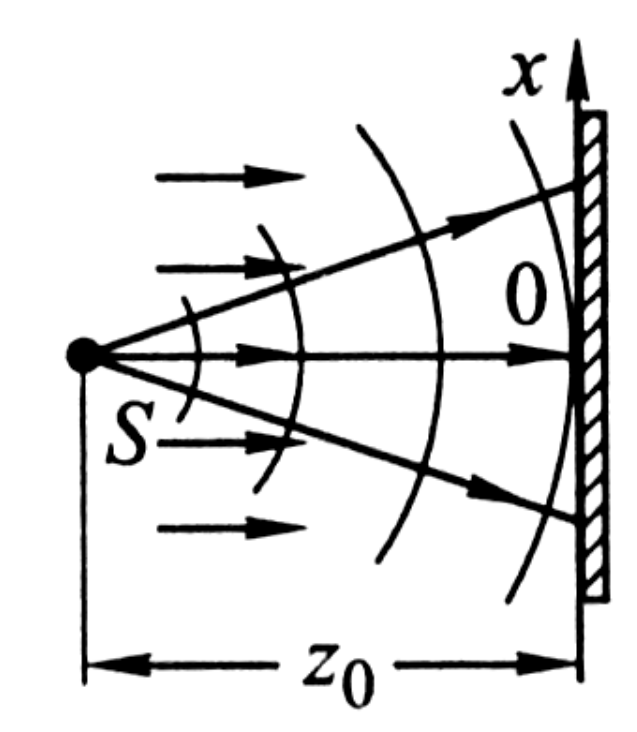
\includegraphics[width=\linewidth]{3.49.png}
  \caption{Запись голограммы точечного источника}
  \label{img::3_49}
\end{wrapfigure}

Для уяснения сути метода рассмотрим в качестве предмета точечный источник света $S$, т.~е. создадим сферическую предметную волну:

$$
f_{\Pi} = \frac{a_{\Pi}}{f} \e^{\iu kr},
$$\\
где $r = \sqrt{z_0^2 + x^2 + y^2}$ ~---~ расстояние от источника $S$ до точки $\left( x, y \right)$ фотопластинки. 

В качестве опорной волны возьмём плоскую волну, бегущую вдоль оси $z$ и падающую нормально на фотопластинку, расположенную в плоскости 
$z = 0$ (рис. \ref{img::3_49}):
$$
f_o = a \e^{\iu kz},
$$\\
т.~е. опорная волна создаёт во всех точках фотопластинки поле одинаковой амплитуды и фазы.

Принимая фазу колебаний в плоскости $z = 0$ равной нулю, запишем $f_о = a$. 
Кроме того, для упрощения формул будем далее полагать, что амплитуда сферической волны во всех точках фотопластинки равна амплитуде плоской волны, 
т.~е. $f_{\Pi} \approx a\e^{\iu kr}$. Суммарное поле в таком случае имеет вид
$$
f = a\e^{\iu kr} + \: a.
$$
\newpage
\begin{wrapfigure}{r}{0.4\linewidth}
  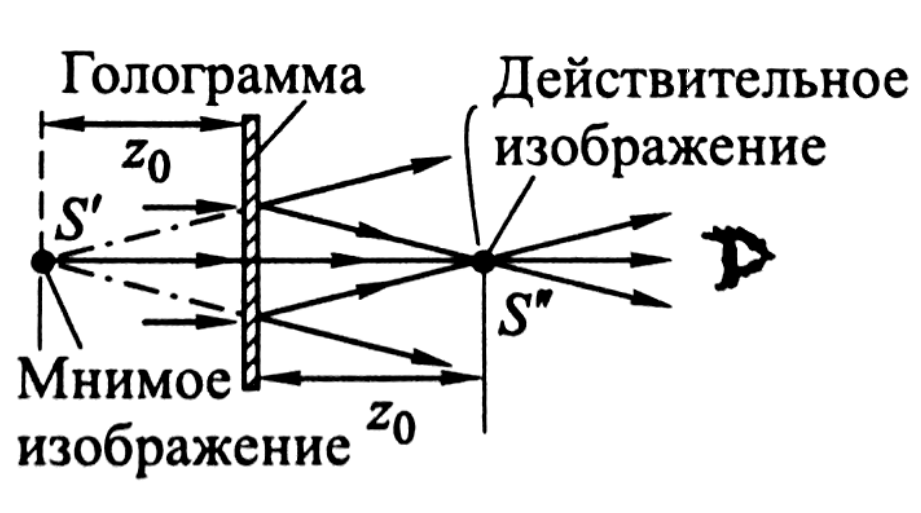
\includegraphics[width=\linewidth]{3.50.png}
  \caption{Восстановление голограммы точечного источника}
  \label{img::3_50}
\end{wrapfigure}
После необходимой фотообработки получаем голограмму с
функцией пропускания:

\begin{equation}\label{eq::3.83}
t\left(x, y\right) \sim I\left(x, y\right)  = 
\left|a +  a\e^{\iu kr}\right|^2.
\end{equation}

Мы описали первую стадию голографического процесса ~---~ процесс записи голограммы.
Теперь необходимо использовать полученную голограмму для восстановления (реконструкции) изображения.

Устанавливаем голограмму в плоскости $z = 0$ и освещаем её плоской нормально падающей волной (рис. \ref{img::3_50}). Для упрощения формул
будем считать амплитуду волны равной единице, а фазу без ограничения общности равной нулю, т.~е. комплексная амплитуда этой волны (её
называют \textbf{восстанавливающей волной}) есть $f_-(x,y) = 1$.

Тогда на выходе голограммы, в плоскости, примыкающей к ней справа, получим
\begin{equation}\label{eq::3.84}
  f_+(x,y) = 1
\end{equation}